%%% LaTeX Template: Article/Thesis/etc. with colored headings and special fonts
%%%
%%% Source: http://www.howtotex.com/
%%% Feel free to distribute this template, but please keep to referal to http://www.howtotex.com/ here.
%%% February 2011
%%%
%%% Modified January 2016 by CDM

%%%  Preamble
\documentclass[11pt,letterpaper]{article}
\usepackage[margin=1.0in]{geometry}
\usepackage[T1]{fontenc}
\usepackage[bitstream-charter]{mathdesign}
\usepackage[latin1]{inputenc}					
\usepackage{amsmath}						
\usepackage{xcolor}
\usepackage{cite}
\usepackage{hyphenat}
\usepackage{graphicx}
\usepackage{float}
\usepackage{subfigure}
\usepackage{sectsty}
\usepackage[compact]{titlesec} 
\usepackage[tablegrid]{vhistory}
\usepackage{pbox}
\allsectionsfont{\color{accentcolor}\scshape\selectfont}

%%% Definitions
\definecolor{accentcolor}{rgb}{0.0,0.0,0.5} 
\newcommand{\teamname}{Resonance}
\newcommand{\productname}{LTunes}
\newcommand{\coursename}{CSE 4316: Senior Design I}
\newcommand{\semester}{Fall 2019}
\newcommand{\docname}{Architectural Design Specification}
\newcommand{\department}{Department of Computer Science \& Engineering}
\newcommand{\university}{The University of Texas at Arlington}
\newcommand{\authors}{Amir Dhungana \\ Anish Yonjan \\ Roberto Torres \\ Raul Jimenez \\ Nikhil Purohit}

%%% Headers and footers
\usepackage{fancyhdr}
	\pagestyle{fancy}						% Enabling the custom headers/footers
\usepackage{lastpage}	
	% Header (empty)
	\lhead{}
	\chead{}
	\rhead{}
	% Footer
	\lfoot{\footnotesize \teamname \ - \semester}
	\cfoot{}
	\rfoot{\footnotesize page \thepage\ of \pageref{LastPage}}	% "Page 1 of 2"
	\renewcommand{\headrulewidth}{0.0pt}
	\renewcommand{\footrulewidth}{0.4pt}

%%% Change the abstract environment
\usepackage[runin]{abstract}			% runin option for a run-in title
%\setlength\absleftindent{30pt}			% left margin
%\setlength\absrightindent{30pt}		% right margin
\abslabeldelim{\quad}	
\setlength{\abstitleskip}{-10pt}
\renewcommand{\abstractname}{}
\renewcommand{\abstracttextfont}{\color{accentcolor} \small \slshape}	% slanted text

%%% Start of the document
\begin{document}

%%% Cover sheet
{\centering \huge \color{accentcolor} \sc \textbf{\department \\ \university} \par}
\vspace{1 in}
{\centering \huge \color{accentcolor} \sc \textbf{\docname \\ \coursename \\ \semester} \par}
\vspace{0.5 in}
\begin{figure}[h!]
	\centering
   	
\includegraphics[width=0.60\textwidth]{images/test_image}
\end{figure}
\vspace{0.5 in}
{\centering \huge \color{accentcolor} \sc \textbf{\teamname \\ \productname} \par}
\vspace{0.5 in}
{\centering \large \sc \textbf{\authors} \par}
\newpage


%\vspace{1 in}
%\centerline{January 13th, 2012}
%\newpage

%%% Revision History
\begin{versionhistory}
  	\vhEntry{0.1}{11.02.2019}{AD}{document creation}
  	\vhEntry{0.2}{11.06.2019}{AY|AD}{complete draft}
  	\vhEntry{1.0}{11.08.2019}{AY|AD}{official release}
\end{versionhistory}
\newpage

%%% Table of contents
\setcounter{tocdepth}{2}
\tableofcontents
\newpage

%%% List of figures and tables (optional)
\listoffigures
\listoftables
\newpage

%%% Document sections
\section{Introduction}
Your introduction should describe your product concept in sufficient detail that the architectural design will be easy to follow. The introduction may include information used in the first sections of your SRS for this purpose. At a minimum, ensure that the product concept, scope and key requirements are described.
\newpage
\section{System Overview}
This section should reintroduce the full data flow diagram from the architectural specification, and discuss at a high level the purpose of each layer. You do not need to include a subsection for each layer, a 1 - 2 paragraph recap is sufficient.

\begin{figure}[h!]
	\centering
 	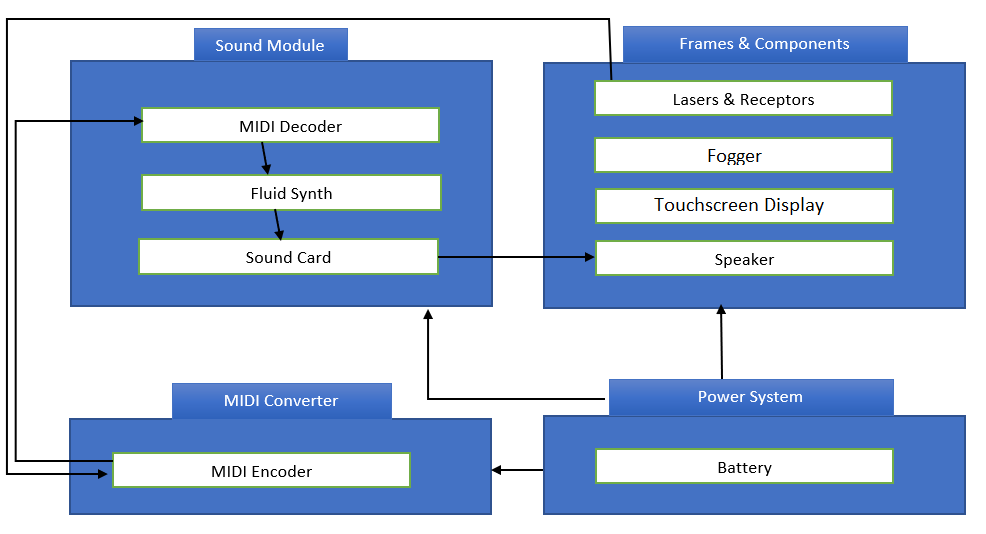
\includegraphics[width=0.90\textwidth]{images/data_flow}
 \caption{System architecture}
\end{figure}

\newpage
\section{Subsystem Definitions \& Data Flow}
This section breaks down your layer abstraction to another level of detail. Here you grapically represent the logical subsytems that compose each layer and show the interactions/interfaces between those subsystems. A subsystem can be thought of as a programming unit that implements one of the major functions of the layer. It, therefore, has data elements that serve as source/sinks for other subsystems. The logical data elements that flow between subsystems need to be explicitly defined at this point, beginning with a data flow-like diagram based on the block diagram.

\begin{figure}[h!]
	\centering
 	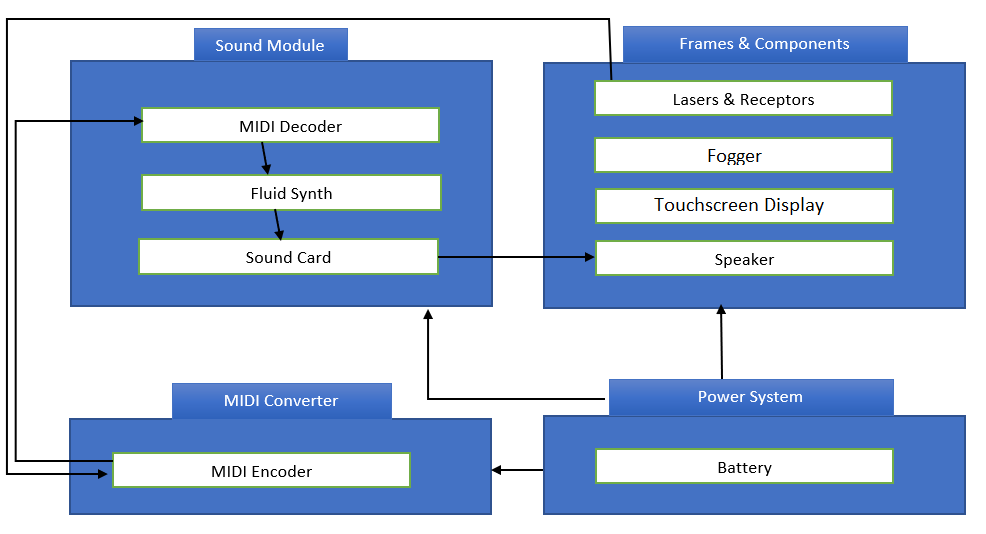
\includegraphics[width=\textwidth]{images/data_flow}
 \caption{A simple data flow diagram}
\end{figure}

\newpage
\section{Power System Layer Subsystems}
This layer is responsible for providing necessary power for the instrument. It mainly consists of 12V 2A DC batteries or regular 120V AC current can be used for this layer.
\subsection{Layer Hardware}
There is no specific hardware required for this layer except of combination 12V batteries and the outlet cord for AC supply . This layer is merely acting as an power source for the raspberry pi, lasers' circuit, teensy micro-controller and mister. 


\subsection{Battery/AC outlet}
It consists of 12V 2A DC batteries' combination or AC outlet along with hookup and jumper wires for connection to the pi and the breadboard.

\begin{figure}[h!]
	\centering
 	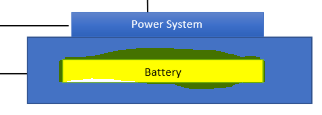
\includegraphics[width=0.60\textwidth]{images/Capture.png}
 \caption{Power layer subsystem diagram}
\end{figure}




\newpage
\section{Frame and Component Layer Subsystems}
In this section, the layer is described in some detail in terms of its specific subsystems. Describe each of the layers and its subsystems in a separate chapter/major subsection of this document. The content of each subsystem description should be similar. Include in this section any special considerations and/or trade-offs considered for the approach you have chosen.

\subsection{Subsystem 1}
This section should be a general description of a particular subsystem for the given layer. For most subsystems, an extract of the architectural block diagram with data flows is useful. This should consist of the subsystem being described and those subsystems with which it communicates.

\begin{figure}[h!]
	\centering
 	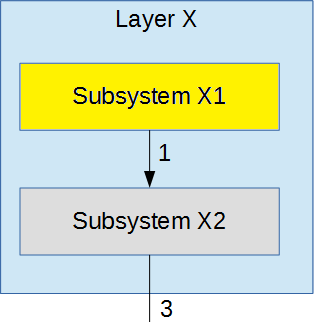
\includegraphics[width=0.60\textwidth]{images/subsystem}
 \caption{Example subsystem description diagram}
\end{figure}

\subsubsection{Assumptions}
Any assumptions made in the definition of the subsystem should be listed and described. Pay particular attention to assumptions concerning interfaces and interactions with other layers.

\subsubsection{Responsibilities}
Each of the responsibilities/features/functions/services of the subsystem as identified in the architectural summary must be expanded to more detailed responsibilities. These responsibilities form the basis for the identification of the finer-grained responsibilities of the layer's internal subsystems. Clearly describe what each subsystem does.

\subsubsection{Subsystem Interfaces}
Each of the inputs and outputs for the subsystem are defined here. Create a table with an entry for each labelled interface that connects to this subsystem. For each entry, describe any incoming and outgoing data elements will pass through this interface.

\begin {table}[H]
\caption {Subsystem interfaces} 
\begin{center}
    \begin{tabular}{ | p{1cm} | p{6cm} | p{3cm} | p{3cm} |}
    \hline
    ID & Description & Inputs & Outputs \\ \hline
    \#xx & Description of the interface/bus & \pbox{3cm}{input 1 \\ input 2} & \pbox{3cm}{output 1}  \\ \hline
    \#xx & Description of the interface/bus & \pbox{3cm}{N/A} & \pbox{3cm}{output 1}  \\ \hline
    \end{tabular}
\end{center}
\end{table}

\subsection{Subsystem 2}
Repeat for each subsystem

\subsection{Subsystem 3}
Repeat for each subsystem


\newpage
\section{Sound Modules Layer Subsystems}
In this section, the layer is described in some detail in terms of its specific subsystems. Describe each of the layers and its subsystems in a separate chapter/major subsection of this document. The content of each subsystem description should be similar. Include in this section any special considerations and/or trade-offs considered for the approach you have chosen.

\subsection{MIDI decoder}
pending
\begin{figure}[h!]
	\centering
 	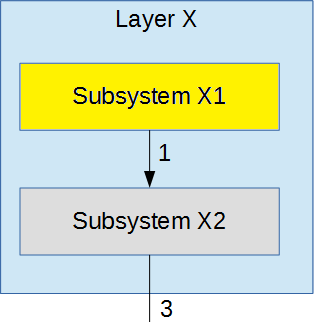
\includegraphics[width=0.60\textwidth]{images/subsystem}
 \caption{Example subsystem description diagram}
\end{figure}

\subsubsection{Assumptions}
pending

\subsubsection{Responsibilities}
pending

\subsubsection{Subsystem Interfaces}
pending

\begin {table}[H]
\caption {Subsystem interfaces} 
\begin{center}
    \begin{tabular}{ | p{1cm} | p{6cm} | p{3cm} | p{3cm} |}
    \hline
    ID & Description & Inputs & Outputs \\ \hline
    \#xx & Description of the interface/bus & \pbox{3cm}{input 1 \\ input 2} & \pbox{3cm}{output 1}  \\ \hline
    \#xx & Description of the interface/bus & \pbox{3cm}{N/A} & \pbox{3cm}{output 1}  \\ \hline
    \end{tabular}
\end{center}
\end{table}

\subsection{Speaker}
The speaker gives the final output of the laser harp. After all the processing of the data in the raspberry pi, the pi sends the final output of the sound signal to the speakers. The speakers produce the desired sound as output. 

\begin{figure}[h!]
	\centering
 	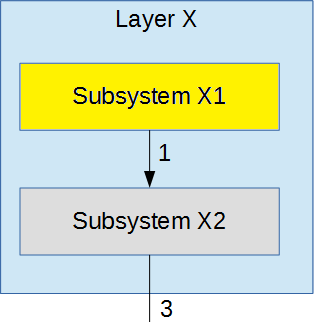
\includegraphics[width=0.60\textwidth]{images/subsystem}
 \caption{Example subsystem description diagram}
\end{figure}

\subsubsection{Assumptions}
The speaker is connected via USB A cable to the pi. It is also powered by the same battery powering the Raspberry Pi.

\subsubsection{Responsibilities}
The speaker should produce decent sound output with no interference. It should be loud enough so the sound can be heard in a conference hall. 

\subsubsection{Subsystem Interfaces}
The speaker gets analog signals from the raspberry pi and converts it into sound waves as output. This is the final output of the system. The speaker is connected via USB A cable to the system.

\begin {table}[H]
\caption {Subsystem interfaces} 
\begin{center}
    \begin{tabular}{ | p{1cm} | p{6cm} | p{3cm} | p{3cm} |}
    \hline
    ID & Description & Inputs & Outputs \\ \hline
    \#xx & Description of the interface/bus & \pbox{3cm}{input 1 \\ input 2} & \pbox{3cm}{output 1}  \\ \hline
    \#xx & Description of the interface/bus & \pbox{3cm}{N/A} & \pbox{3cm}{output 1}  \\ \hline
    \end{tabular}
\end{center}
\end{table}

\subsection{FluidSynth}
FluidSynth is a real-time software synthesizer based on the SoundFont 2 specifications and has reached widespread distribution. It converts the MIDI signals to produce desired sound waves.

\begin{figure}[h!]
	\centering
 	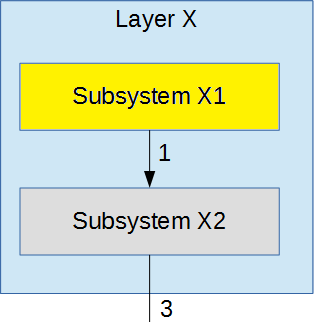
\includegraphics[width=0.60\textwidth]{images/subsystem}
 \caption{Example subsystem description diagram}
\end{figure}

\subsubsection{Assumptions}
The software already has default preset sounds built-in. It also has the functionality manipulate the sound to produce various sound effects. Also it is free, open source and easy to use.

\subsubsection{Responsibilities}
The software is used to convert MIDI signals to sound waves. It should have multiple different sound effects and create a wide range of sound octaves in different formats.

\subsubsection{Subsystem Interfaces}
The software is downloaded and installed into the raspberry pi. It is supported by the Raspian OS.

\begin {table}[H]
\caption {Subsystem interfaces} 
\begin{center}
    \begin{tabular}{ | p{1cm} | p{6cm} | p{3cm} | p{3cm} |}
    \hline
    ID & Description & Inputs & Outputs \\ \hline
    \#xx & Description of the interface/bus & \pbox{3cm}{input 1 \\ input 2} & \pbox{3cm}{output 1}  \\ \hline
    \#xx & Description of the interface/bus & \pbox{3cm}{N/A} & \pbox{3cm}{output 1}  \\ \hline
    \end{tabular}
\end{center}
\end{table}

\newpage
\section{MIDI Layer Subsystems}
In this section, the layer is described in some detail in terms of its specific subsystems. Describe each of the layers and its subsystems in a separate chapter/major subsection of this document. The content of each subsystem description should be similar. Include in this section any special considerations and/or trade-offs considered for the approach you have chosen.

\subsection{MIDI encoder}
The MIDI encoder gets the signal from the laser receptors, converts it to MIDI data and sends to the Raspberry Pi for the output. This converts the laser receptor signals to MIDI data in order to convert it to sound data.  

\begin{figure}[h!]
	\centering
 	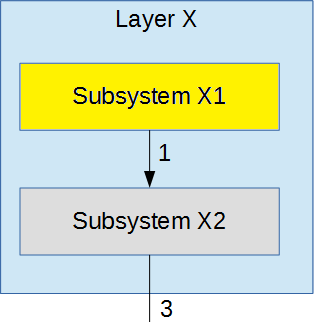
\includegraphics[width=0.60\textwidth]{images/subsystem}
 \caption{MIDI encoder subsystem description diagram}
\end{figure}

\subsubsection{Assumptions}
The MIDI encoder is connected to the Pi and the laser receptors via usb-A cable. It also has a built-in software that converts the data automatically.

\subsubsection{Responsibilities}
The laser recptors, when it detects an interference, sends signal to the MIDI encoder. Here, the encoder converts the signal data it received to a MIDI data so it can be maniplated to different sounds with the sound modules.

\subsubsection{Subsystem Interfaces}
Each of the inputs and outputs for the subsystem are defined here. Create a table with an entry for each labelled interface that connects to this subsystem. For each entry, describe any incoming and outgoing data elements will pass through this interface.

\begin {table}[H]
\caption {Subsystem interfaces} 
\begin{center}
    \begin{tabular}{ | p{1cm} | p{6cm} | p{3cm} | p{3cm} |}
    \hline
    ID & Description & Inputs & Outputs \\ \hline
    \#xx & Description of the interface/bus & \pbox{3cm}{input 1 \\ input 2} & \pbox{3cm}{output 1}  \\ \hline
    \#xx & Description of the interface/bus & \pbox{3cm}{N/A} & \pbox{3cm}{output 1}  \\ \hline
    \end{tabular}
\end{center}
\end{table}



\newpage

%%% References
\bibliographystyle{plain}
\bibliographystyle{reference/IEEEtran_custom}
\bibliography{reference/refs}{}

\end{document}
